% code against the government vote
% produce a data.key
% how does Bundesrat decide on vote recommendation
% average sample size (and sd) 
% bias: overreporting of turnout, bandwaggoning, social desirability: it not socially desirable to vote for certain initiatives
% Is there underreporting of against the government votes?

\documentclass[11pt,a4paper]{article}
\usepackage[utf8]{inputenc}
\usepackage{amsmath}
\usepackage{amsfonts}
\usepackage{amssymb}
\usepackage{graphicx}
\usepackage[round]{natbib}
\usepackage{url}
\usepackage{graphicx}
\usepackage{setspace}

\author{Arndt Leininger \thanks{Hertie School of Governance, \texttt{a.leininger@phd.hertie-school.org}}}
\title{\Large{\textsc{Who votes against the government and why?}}\\ \large{\textsc{Voting Behavior in National Referendums in Switzerland}}} % Change title?
\date{\today}

\onehalfspacing

\begin{document}

\maketitle

{\small \textit{Contribution to the Leuven-Montréal Winter School in Elections and Voting Behaviour 2015. Current draft and code at:} \texttt{github.com/aleininger/votingreferendums}}



\begin{abstract}
	
	This paper studies voting behavior in national referendums in Switzerland, more concretely what motivates voters to vote counter to the vote recommendations issued by the Swiss federal government.
\end{abstract}	

\small\textbf{Keywords: Referendums, Voting, Switzerland, Multi-level modelling}

\vfill

\newpage

\section{Introduction}\label{sec:introduction}

    Voters vote in referendums more often and in more places than is commonly thought. Yet, voting in referendums has largely been a neglected topic in research on voting behavior which mostly focused on electoral behavior. The research that exists has focused on whether citizens are capable of casting an informed vote as levels of voter competence in referendums are thought to be even lower than in elections. This line of research has, counter to popular arguments against direct democracy, found that even uninformed citizens often are capable to vote in a way they would have voted had they been better informed on the issue at hand. Low-informed  voters are able to mimic informed voters' choices by relying on cues from governments, parties and interest groups.
    
    This paper is motivated by the observation that in Switzerland the effectiveness of such cues, concretely vote recommendations propagated by the Swiss government, has apparently decreased in effectiveness. Switzerland has since roughly the late 1970s experienced a secular upward trend in the number of referendums the government loses, both in absolute and relative terms (Fig. \ref{fig}). The initiatives on a ban on building minarets in 20xx and the deportation of convicted non-Swiss citizens in 20xx which were both opposed by the government but still approved by a majority of voters are only two prominent examples from recent times.
    
    I use the full cumulation of the VOX post-referendum surveys that cover all 246 national referendums held in Switzerland between 1981 and 2010 to analyze the individual and macro-level determinants of voting `against the government.' Given the state of the literature on referendum voting the paper is rather descriptive in nature. I focus on identifying the determinants of the above defined outcomes rather than precisely estimating a specific determinant. As detailed in section \ref{sec:litreview} established determinants of electoral choice cannot be readily adapted to studies of vote choice in referendums and expected to work the same way. 
    
    On the individual level I concentrate on citizens' political competence -- capturing how informed voters are about a referendum -- and political sophistication more generally -- how interested and informed citizens are about politics in general. In include the usual socio-economic covariates which in Switzerland include the politico-linguistic divide between the German and the French and to a lesser degree the Italian speaking Swiss population. 
    
    On the macro level I spotlight the type and topic of a referendum as well as the campaign waged by proponents and opponents in the lead-up to a referendum. While obligatory referendums are triggered by government action initiatives are a tool for interest groups to enact policies the legislature would not pass. Who triggers a referendum could have an effect on citizens' propensity to reject the policy favored by the government. On the topics considered in a referendum it has been suggested by many commentators that initiatives directed against minorities have proven particularly successful. Of particular relevance to parties and governments, lastly, is the question whether campaigns can encourage citizens to vote in the desired way.
    
    Following the presentation of initial results, I will also outline two potential extensions to the paper. Firstly, I articulate thoughts on how one could, among the voters `defying' the government, distinguish what I would call `reasoned' from `populist' deviators.  
    
    Secondly, I discuss how an analysis of individual voting behavior could contribute to explaining the macro-level trend in rising numbers of government defeats. This trend could be rooted in both macro and individual level factors. For instance, if voters are more likely to vote against the government's recommendation if the referendum was triggered by an initiative then the recent rise in initiatives on the ballot (Fig. \ref{fig}) could explain part of the increase in `defeats.' On the individual level, a decline in party identification in the voting population could explain why voters increasingly disregard their government's vote advice.

\begin{figure}[htb]
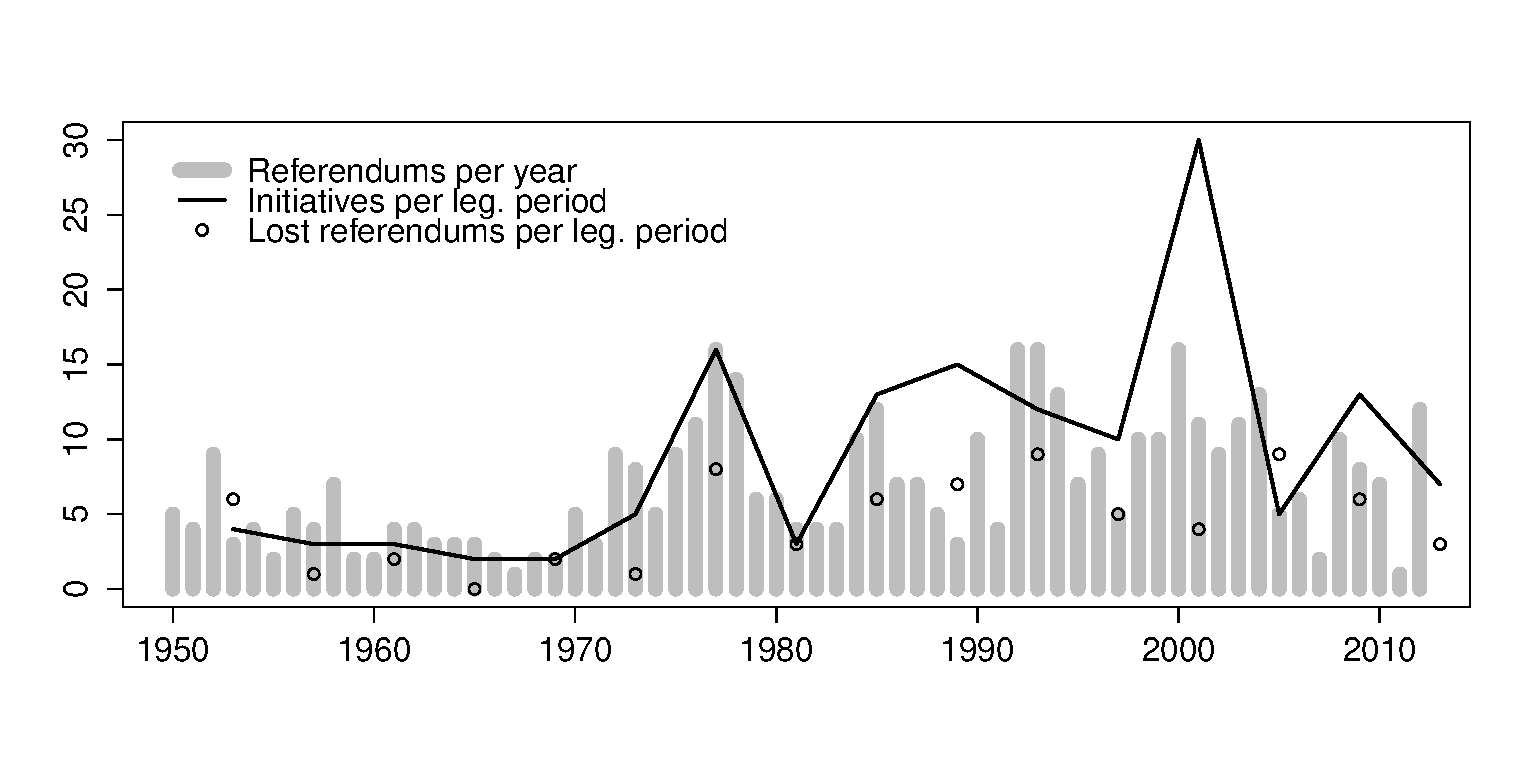
\includegraphics[width=\textwidth]{../../figures/figure.pdf}    
\caption{Number of national referendums, initiatives and referendums lost by the government in Switzerland (1950-2013). Counts per legislative period plotted at midpoint of legislative period.}\label{fig}
\end{figure}

\section{Literature review}\label{sec:litreview}

	The literature on voting behavior is immense with highly specialized sub-topics. literature reviews have to focus on the most immediately relevant papers in a given subfield of electoral behavior. 
	
	The literature on voting behavior largely is a literature of electoral behavior. review much more scattered. odd collection of empirical cases outcomes of interest.
	
	Before providing a sketch of the literature, outline some of the reasons why referendums have received little attention in the voting literature. 
	
	substantive and practical reasons.
	
	Substantively, referendums have been of great appeal to theorists as embodiment of democracy, yet because of their lack of prominence in actual politics been of lesser interest. This has changed in recent years. increase in referendums globally. Extension of institutionalization. uptake in use and academic interest do not perfectly coincide as preliminary high point of use was in 90s(?). Greater role in politics, discussions of political reform. also explains academic interest.
		
	Practical reasons. no data available. referendums occur infrequently and most often, outside of Switzerland, on the subnational level. Not many surveys. While every national and many subnational elections are accompanied by scientific election surveys scientific surveys on referendums are much rarer. 
	
	For this reason much research has been on aggregate level. Relating referendum outcomes to other macro level factors. not focus of this literature review which focuses on individual level.
	
	Schoen (2012) cautions that determinants of electoral and referendum participation differ, determinants of vote choice differ even more between elections and referendums. 
	
	offers reasons:
	
%	"Solche von Bürgern initiierte Abstimmungen
%	beziehen sich häufig auf Forderungen, die in der repräsentativdemokratischen Arena keine
%	Mehrheit oder sogar überhaupt kein Gehör gefunden haben, und bringen insofern
%	Repräsentationsschwächen der zentralen repräsentativdemokratischen Akteure, also
%	vornehmlich der Parteien, zum Ausdruck. Daher ist es wohl kein Zufall, wenn bei
%	Volksentscheiden dieser Art andere politische Konfliktlinien und andere kollektive Akteure
%	als in der repräsentativdemokratischen Arena eine herausragende Rolle spielen" (Schoen 2012, S. 5)

referendums, initiatives, are used for proposal that found no majority in representative system or were not sufficiently addressed. referendums can be used by representative to 'outsource' contentious issues to the electorate. 

Other societal actors become more prominent. 

referendums vote on one issue as opposed to parties fundamentally different in essence. different context. regularities in electoral behavior cannot expected to appear in referendum voting.

even holds for strong determinants like party identification. If parties refrain from campaigning paty identification will play less role in determining vote choice. Schoen (2012) illustrates this where campaing was dominated by two interest groups.

\section{sec:theory}

Michigan: party identification issue and candidate orientation. 

there are no parties or candidates to elect, only an issue to decide. issue much more prominent. Party identification and 

every election is unique. voting research focuses on abstractions. voting for incumbent, for a left party, ticket-splitting. abstraction to be comparative and cumulative. but parties on offer are stable across elections. make sense to investigate vote choice for social democrats. develop an understanding how this might have changed. clear categories like government.

referendums are arguably more difficult to put into an analytical framework that is amenable to a comparative and cumulative referendum.

Here the proposal and proposer vary from referendum to referendum. 
Define an outcome variable that is consistent across referendums. Voting no, status quo bias. to a certain degree. but initiative no is pro status quo, in a facultative referendum not so clear, reversal of policy back to an older status quo. whether voters voted correctly. 

voters voted against government. normatively important. institution seems to be directed against representative process. a successful referendum is defeat for government. tool for populists.

normvatively interesting.

take note of recent increase in government losses.

What motivates citizens to vote against government.

discuss these. literature is limited. instead of formulating hypothesis only questions.

\textbf{Q1} Are deviators less informed than voters voting with the government?

My approach is descriptive in nature. I focus on identifying determinants of the above defined outcomes rather than precisely estimating a specific determinant. Interesting correlations. should not be treated causal (Keele paper). For instance, the inclusion of political knowledge in the regression models is motivated by the normatively and politically important question whether voters are less well informed than others. It is not motivated by the questions whether lack of knowledge causes voting against the government.

\section{Data \& Empirics}

246 referendums. representative at the national level. average sample size of 

As in most studies there is overreporting of turnout. Is there underreporting of against the government votes?

\section{Results}

\section{Conclusions}

\textit{To be included in future revision.}


\end{document}
